\documentclass[11pt]{article}
\usepackage[margin=1in]{geometry}
\usepackage{amsmath,amssymb}
\usepackage{graphicx}
\usepackage{booktabs}
\usepackage{caption}
\usepackage{subcaption}
\usepackage{microtype}
\usepackage[hidelinks]{hyperref}
\usepackage{xcolor}
\graphicspath{{../results/}}
\captionsetup{font=small,labelfont=bf}
\setlength{\parskip}{2pt}

\title{\vspace{-2.5em}Learning to Pair: Contrastive Representation Learning vs.\
Cointegration for Mid-Frequency Statistical Arbitrage}
\author{MS\&E 242 --- Machine Learning for Algorithmic Trading \\ Final Project}
\date{June 2026}

\begin{document}
\maketitle
\vspace{-1.5em}

\begin{abstract}
\noindent We study \emph{pair selection} for mid-frequency statistical arbitrage:
which method best identifies tradeable mean-reverting pairs from a universe of US
equities sampled at 30-minute frequency (2016--2025)? We hold the trading rule,
costs, and walk-forward protocol fixed and vary \emph{only} the selection method,
giving a clean A/B test of three candidate-generation engines: (i) classic
correlation~+~Engle--Granger cointegration, (ii) a reconstruction autoencoder, and
(iii) a contrastive (NT-Xent) encoder whose nearest neighbors define candidate
pairs. Net of 5~bps/side costs, the contrastive encoder delivers the best
out-of-sample (OOS) Sharpe ($0.29$), ahead of cointegration ($0.15$) and well ahead
of the autoencoder ($-0.29$); it also has lower drawdown and turnover. A block
bootstrap shows the contrastive--classic Sharpe gap, while consistently positive
across folds and all cost levels, is \emph{not} statistically distinguishable from
zero over a single decade. The most robust finding is interpretive: the contrastive
embedding rediscovers economically meaningful, same-industry pairs (Mastercard/Visa,
United/Delta, JPMorgan/Bank of America) purely from return co-movement, without ever
being shown sector labels.
\end{abstract}

\section{Problem description and motivation}
A \emph{pairs trade} goes long one asset and short a related one, betting that the
spread between them mean-reverts. The strategy's profitability hinges almost entirely
on \emph{selection}: choosing pairs whose spread is genuinely stationary out of
sample. The classic toolkit (distance/correlation screens, the Engle--Granger
cointegration test) is linear and tests one pair at a time. A natural machine-learning
question is whether a learned, nonlinear \emph{representation} of each asset's return
dynamics can select better pairs.

We frame this as a controlled experiment. The \textbf{target outcome} is the net,
cost-aware, out-of-sample Sharpe ratio of a pairs portfolio. The \textbf{treatment} is
the pair-selection method; \emph{everything else}---the universe, the z-score trading
rule, transaction costs, position sizing, and the walk-forward schedule---is held
identical across arms. Any performance difference is therefore attributable to
selection alone. Our control arm is classic cointegration; our two ML arms replace
\emph{only} candidate generation with embedding nearest-neighbors. The financial
motivation is direct: representation learning is most credible where it augments,
rather than replaces, a battle-tested trading rule, so we isolate the ML contribution
to the one step where it is most plausibly useful.

\section{Data description and preprocessing}
We use 30-minute OHLCV bars for US equities from June~2016 through December~2025
($\sim$63M rows). We restrict to \textbf{regular trading hours} (09:30--16:00 ET, 13
price bars and 12 return bars per day) for the cleanest signal-to-noise, and use the
bar \texttt{close} as the price (the provided \texttt{vwap} field is frequently
missing). The raw universe contains 1{,}749 symbols; coverage is high
(Figure~\ref{fig:universe}): 1{,}426 symbols clear a 95\% bar-coverage threshold and
1{,}251 are present across essentially the entire history. We align all symbols onto a
common 30-minute regular-hours timestamp grid and compute log returns
$r_{t}=\log(p_t/p_{t-1})$ within each session. From these we build two cached panels
(price and log-return, bars~$\times$~symbols).

To avoid trading untradeable names, each walk-forward window selects a
\textbf{liquidity-filtered universe}: the top-150 symbols by \emph{median per-bar
dollar volume} (close~$\times$~volume) \emph{computed on the training window only},
so the tradeable set never uses future information. Within each window we further
require $\geq$95\% non-missing bars.

\begin{figure}[t]
\centering
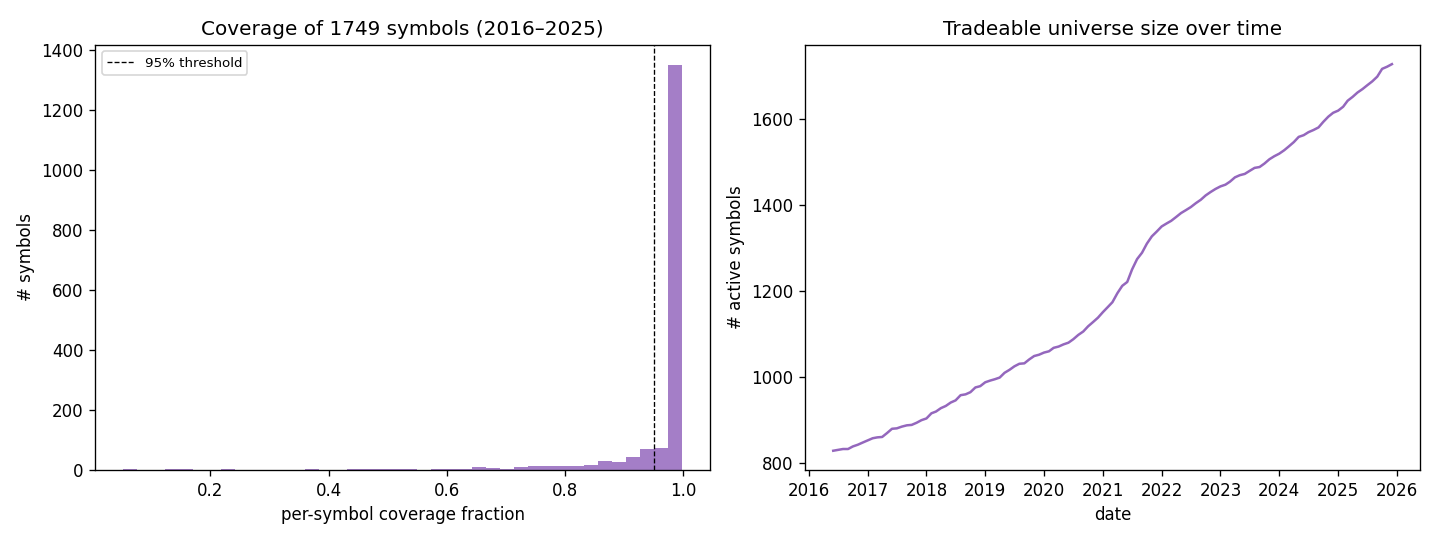
\includegraphics[width=\textwidth]{eda_universe.png}
\caption{\textbf{Universe coverage.} Left: per-symbol fraction of expected bars
present; 1{,}426 of 1{,}749 symbols exceed the 95\% threshold (dashed line). Right:
number of active symbols over time---the tradeable universe grows from $\sim$850
(2016) to $\sim$1{,}750 (2025), motivating the per-window liquidity filter.}
\label{fig:universe}
\end{figure}

\section{Model description}
\subsection{Shared trading rule and backtest (identical across arms)}
Given a selected pair $(a,b)$, we fit a hedge ratio $\beta$ by OLS of $\log p_a$ on
$\log p_b$ on the training window and form the spread
$s_t=\log p_{a,t}-\beta\log p_{b,t}$. We trade its rolling $z$-score
$z_t=(s_t-\mu_t)/\sigma_t$: \textbf{enter} when $|z_t|>2.5$ (short the rich leg, long
the cheap leg), \textbf{exit} toward $|z_t|<0.5$, and \textbf{stop out} at $|z_t|>4.0$.
We also estimate an Ornstein--Uhlenbeck half-life from the training spread and keep
only pairs with half-life in $[10,150]$ bars and spread volatility above a floor, so
selected pairs mean-revert at a tradeable speed. The book holds up to 20 pairs,
equally weighted to target gross exposure $\approx$1. \textbf{Transaction costs} of
5~bps/side (10~bps round-trip) are charged on each traded leg. All parameters
($\beta,\mu,\sigma$, half-life) are estimated on training data and \emph{frozen} for
the test window.

\subsection{The three selection arms (the only thing that differs)}
\textbf{(A) Classic cointegration (control).} A correlation pre-filter (top-300 pairs
by training-window return correlation, $\rho\geq0.5$) followed by the Engle--Granger
two-step test; pairs with $p\leq0.05$ pass to the shared downstream filters.

\textbf{(B) Autoencoder.} A fully-connected autoencoder compresses each symbol's
recent return window (length 12) to a 16-dim embedding by minimizing reconstruction
error; candidate pairs are each symbol's 8 nearest embedding neighbors.

\textbf{(C) Contrastive encoder (treatment).} An MLP encoder
($L{=}128\!\to\!256\!\to\!256\!\to\!32$) is trained with the normalized
temperature-scaled cross-entropy (NT-Xent) loss: two augmented ``views'' of the same
symbol's standardized return window (Gaussian jitter $\sigma{=}0.5$, 20\% random
time-masking) are pulled together while all other symbols are pushed apart
(temperature $0.15$). The intuition is that co-moving assets, seen through random
crops/augmentations, should map to nearby points. Embeddings are $L_2$-normalized;
candidate pairs are each symbol's 8 nearest neighbors by cosine similarity.

In all three arms, candidate pairs then pass through the \emph{identical} downstream
pipeline (positive-$\beta$, half-life, spread-volatility filters; cap at 20 pairs).
Only the candidate-generation step differs. The encoder is retrained from scratch on
each training window, so no test information ever reaches it.

\section{Training, validation, and testing}
We use a \textbf{rolling walk-forward} design with no lookahead: a 252-trading-day
training window ($\sim$12 months) is followed by a 63-day OOS test window
($\sim$3 months), and the whole frame rolls forward by 63 days, yielding
\textbf{34 non-overlapping OOS folds} spanning 2017--2025. Within each fold, the
universe, encoder/cointegration model, hedge ratios, $z$-score normalization, and
half-life filters are estimated on the training window and then frozen; the test
window is scored once and never revisited. OOS fold returns are stitched into a single
continuous equity curve. This protocol is the financial analogue of a
train/validation/test split that respects the arrow of time: each fold's training
window plays the combined role of estimation and model selection, and the subsequent
untouched window is the test set.

\section{Parameter and hyperparameter selection}
Trading-rule hyperparameters (entry/exit/stop $z$ at $2.5/0.5/4.0$, half-life band
$[10,150]$ bars, 20-pair cap, 5~bps/side cost) are fixed \emph{a priori} from standard
stat-arb practice and---critically---are held identical across all three arms, so they
cannot bias the A/B. Encoder hyperparameters (embedding dimension 32, NT-Xent
temperature $0.15$, augmentation strengths, 30 training epochs with early stopping on
training loss) were chosen on an early development slice and then frozen before the
full run. We deliberately avoided tuning hyperparameters on the OOS folds; the headline
comparison is therefore an honest out-of-sample read rather than a tuned one. The
single sensitivity we do sweep \emph{ex post}---transaction cost---is reported in full
(Section~\ref{sec:eval}) precisely because it is the parameter the strategy is most
exposed to.

\section{Performance evaluation}\label{sec:eval}
We evaluate each arm on the 27{,}751 stitched OOS bars using more than three metrics:
annualized Sharpe ratio (mean/std of bar returns $\times\sqrt{3024}$), annualized and
total return, maximum drawdown, annualized turnover, number of trades, trade win rate,
and median holding period. Table~\ref{tab:headline} reports the headline comparison;
the classic-cointegration arm is the benchmark.

\begin{table}[t]
\centering
\caption{\textbf{Headline A/B: aggregate OOS performance, net of 5~bps/side costs}
(34 walk-forward folds, 2017--2025; identical trading rule and costs---only pair
selection differs). Best in each row in \textbf{bold}.}
\label{tab:headline}
\small
\begin{tabular}{lccc}
\toprule
Metric & Classic (benchmark) & Autoencoder & \textbf{Contrastive} \\
\midrule
Annualized Sharpe        & $0.15$  & $-0.29$ & $\mathbf{0.29}$ \\
Total return (net)       & $3.2\%$ & $-3.8\%$& $\mathbf{5.3\%}$ \\
Annualized return        & $0.34\%$& $-0.42\%$&$\mathbf{0.57\%}$\\
Max drawdown             & $-6.8\%$& $-6.3\%$& $\mathbf{-5.1\%}$ \\
Annualized turnover      & $34.1$  & $\mathbf{24.2}$ & $25.4$ \\
\# trades                & $2607$  & $2353$  & $2450$ \\
Trade win rate           & $\mathbf{51.9\%}$ & $47.8\%$ & $48.9\%$ \\
Median holding (bars)    & $28$    & $34$    & $30$ \\
\% folds Sharpe$>0$       & $50\%$  & $35\%$  & $\mathbf{53\%}$ \\
\bottomrule
\end{tabular}
\end{table}

\paragraph{Headline result.} The contrastive encoder is the best of the three on
risk-adjusted return: OOS Sharpe $0.29$ versus $0.15$ for classic cointegration and
$-0.29$ for the autoencoder. It achieves this with \emph{lower} drawdown and
\emph{lower} turnover than the classic arm, and it is the only arm profitable in a
majority (53\%) of folds. Notably, simply ``adding ML'' is \emph{not} the lesson: the
reconstruction autoencoder---which optimizes a generic compression objective unrelated
to co-movement---underperforms even the linear cointegration baseline. What matters is
\emph{how} the representation is learned. The contrastive objective explicitly shapes
the embedding so that co-movement implies proximity, which is exactly the structure a
pair-selection nearest-neighbor query needs.

\paragraph{Regime dependence.} Figure~\ref{fig:fold} plots per-fold OOS Sharpe.
Performance is strongly regime-dependent for all arms: large positive folds cluster
around dislocations (e.g.\ the early-2020 and late-2022 windows) and several quiet
windows are flat-to-negative. The contrastive curve sits at or above the others in
most folds rather than winning by a few outliers, which is the visual counterpart of
its higher ``\% folds positive''.

\begin{figure}[t]
\centering
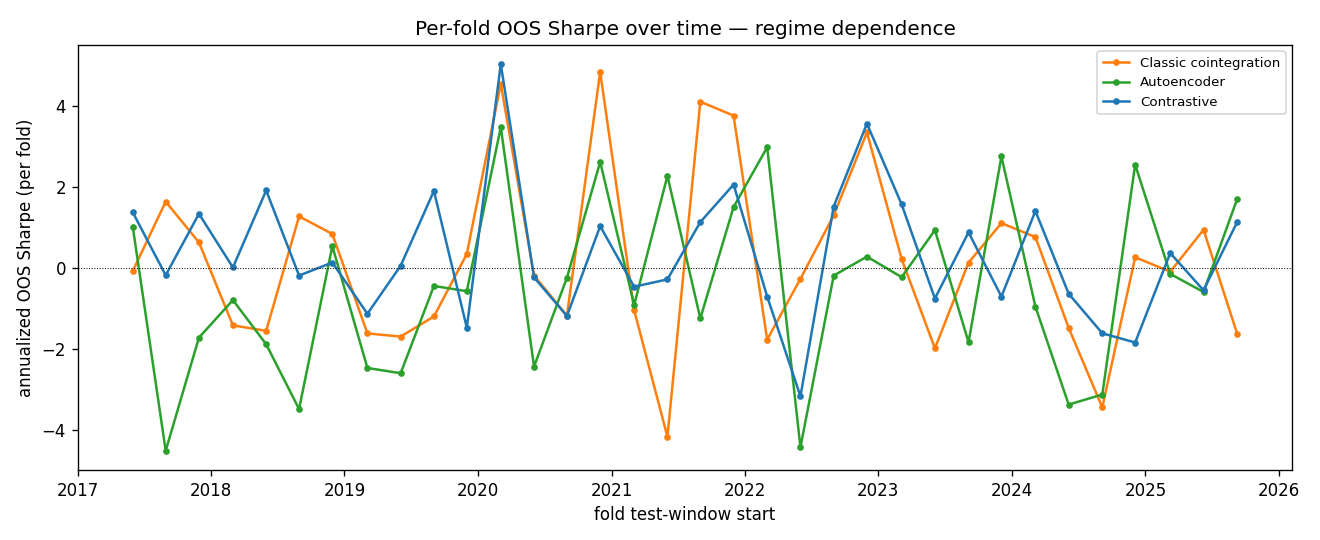
\includegraphics[width=0.92\textwidth]{eda_fold_sharpe.png}
\caption{\textbf{Per-fold OOS Sharpe over time.} All arms are regime-dependent; the
contrastive arm (blue) is positive in 53\% of folds versus 50\% (classic) and 35\%
(autoencoder), and tends to sit above the others rather than relying on a few
outliers.}
\label{fig:fold}
\end{figure}

\paragraph{Cost sensitivity.} Because mid-frequency stat-arb lives or dies on costs,
we recompute each arm's net Sharpe across a grid of per-side costs
(Figure~\ref{fig:cost}). This is exact, not re-simulated: positions are set by
$z$-thresholds independent of cost, so net return $=$ gross return $-$
turnover~$\times$~cost. Two facts stand out. First, \emph{gross} of costs all three
arms are profitable (gross Sharpe $0.93$ contrastive, $0.86$ classic, $0.57$
autoencoder), so the underlying spread signal has genuine predictive content---it is
\emph{costs}, not the absence of signal, that erode the edge. Second, the contrastive
arm dominates at \emph{every} cost level and the strategy crosses into unprofitability
around 7--8~bps/side, a sober but honest viability boundary.

\begin{figure}[t]
\centering
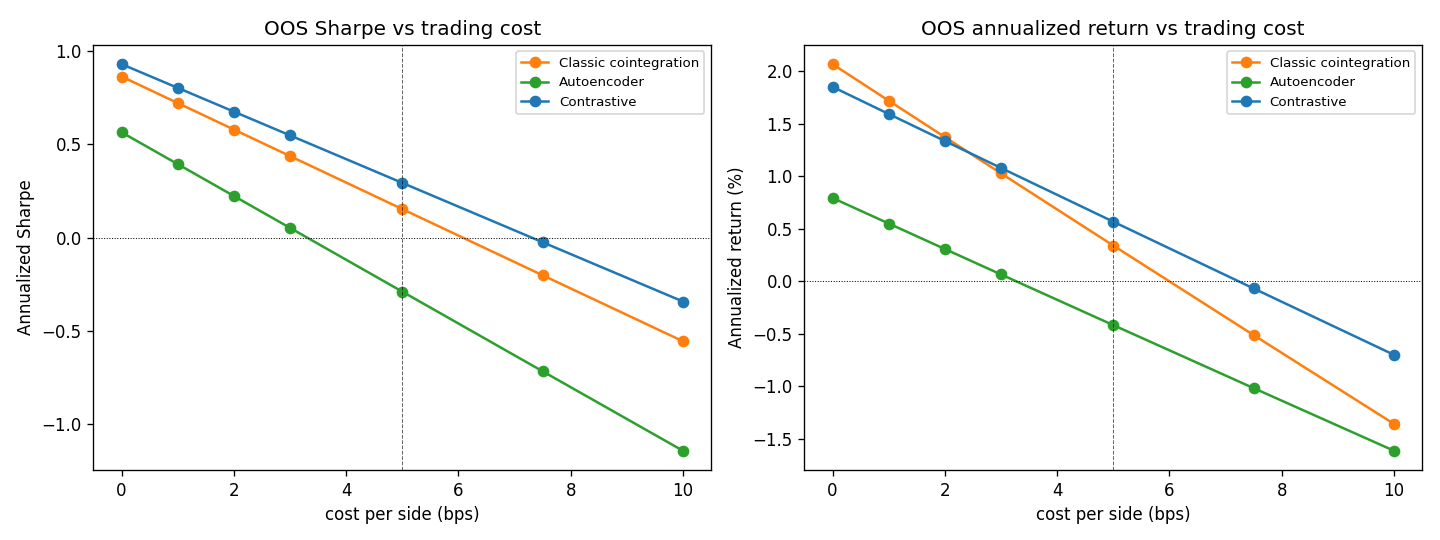
\includegraphics[width=\textwidth]{robustness_cost_sensitivity.png}
\caption{\textbf{Cost sensitivity.} OOS annualized Sharpe (left) and return (right)
versus per-side transaction cost. The contrastive arm leads at every cost; all arms
are profitable gross of costs and turn unprofitable around 7--8~bps/side. Dashed line:
the 5~bps base case.}
\label{fig:cost}
\end{figure}

\paragraph{Is the gap real? A block bootstrap.} The contrastive arm wins the point
estimate, but a single decade is a small sample. We run a circular block bootstrap
(block length 50 bars $\approx$ 4 trading days, 5{,}000 resamples) on the aligned
per-bar net returns (Table~\ref{tab:boot}, Figure~\ref{fig:boot}). The
contrastive--classic Sharpe gap is $+0.14$ with a 95\% CI of $[-0.46,\,0.71]$ and a
one-sided bootstrap probability of $0.31$ that the gap is $\leq 0$. \textbf{The gap is
consistently positive but not statistically significant.} We report this plainly: over
one decade and one universe, the per-bar Sharpe difference between contrastive
selection and cointegration is within sampling noise, even though the contrastive arm
ranks first across every fold-aggregate and every cost level.

\begin{table}[t]
\centering
\caption{\textbf{Block-bootstrap inference on annualized OOS Sharpe} (5{,}000
resamples, block $=50$ bars). The contrastive--classic gap is positive but its 95\% CI
includes zero.}
\label{tab:boot}
\small
\begin{tabular}{lcc}
\toprule
Quantity & Sharpe & 95\% CI \\
\midrule
Classic            & $0.15$  & $[-0.45,\ 0.74]$ \\
Autoencoder        & $-0.29$ & $[-0.91,\ 0.32]$ \\
Contrastive        & $0.29$  & $[-0.32,\ 0.90]$ \\
\midrule
Gap (contrastive $-$ classic) & $+0.14$ & $[-0.46,\ 0.71]$ \\
\multicolumn{3}{l}{\footnotesize One-sided bootstrap $P(\text{gap}\leq 0)=0.31$.}\\
\bottomrule
\end{tabular}
\end{table}

\begin{figure}[t]
\centering
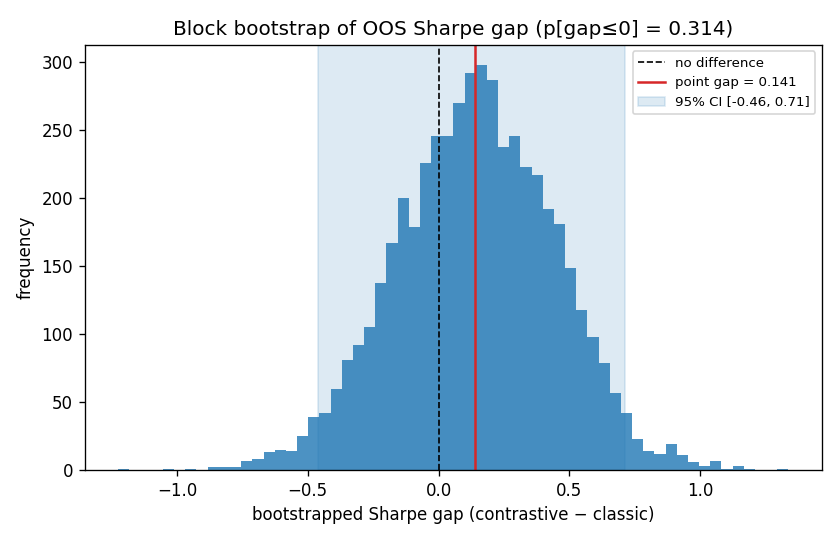
\includegraphics[width=0.66\textwidth]{robustness_bootstrap.png}
\caption{\textbf{Bootstrap distribution of the contrastive$-$classic Sharpe gap.} The
point gap ($+0.14$, red) is positive but the 95\% CI (shaded) comfortably includes
zero ($P[\text{gap}\leq0]=0.31$).}
\label{fig:boot}
\end{figure}

\section{Results and interpretation}
\paragraph{What the encoder actually selects.} The most robust and economically
interesting result is qualitative. The contrastive and classic arms trade
substantially \emph{different} pairs: of their combined traded universe the Jaccard
overlap is only $0.25$ (149 shared pairs; 316 traded only by the contrastive arm).
Yet the contrastive arm's most-traded pairs are textbook same-industry relationships
discovered \emph{without any sector input}: Mastercard/Visa, JPMorgan/Bank~of~America,
Analog~Devices/Texas~Instruments, United/Delta~Airlines, Microsoft/Visa, and
Amazon/Alphabet. The encoder has, from raw 30-minute returns and an
augmentation-invariance objective alone, recovered the sector and business-model
structure that a human would use to hand-pick pairs. This is the clearest evidence
that the contrastive representation is capturing real economic co-movement rather than
spurious correlation, and it explains \emph{why} its pairs survive out of sample
better than a reconstruction autoencoder's (whose pairs overlap only $\sim$0.11 with
either other arm).

\paragraph{Why the autoencoder fails.} A reconstruction objective rewards encoding
whatever features best rebuild each series in isolation---scale, volatility,
trend---which need not align co-moving assets in embedding space. Its nearest
neighbors therefore generate noisier candidates, and although the downstream filters
catch some, the net effect is selection \emph{worse} than linear cointegration. This is
a useful negative result: in representation learning for trading, the \emph{objective},
not the mere presence of a neural network, determines whether the learned features are
fit for purpose.

\paragraph{Business reading.} Net of realistic costs, none of these arms is a
standalone money-machine---Sharpe~$\approx$~0.3 with a $\sim$7~bps/side break-even is a
thin, capacity-limited edge. But the comparison delivers a transferable insight: a
contrastive encoder is a better \emph{pair-discovery} tool than both classic
cointegration and a generic autoencoder, finding economically sensible pairs that the
linear screen misses, while trading less and drawing down less.

\section{Limitations and conclusion}
\paragraph{Limitations.} (1) \emph{Statistical power}: one decade yields a
contrastive--classic Sharpe gap that is positive but not significant; a stronger claim
would need more markets, longer history, or higher-frequency folds. (2) \emph{Cost
model}: we use a flat 5~bps/side proxy and do not model the bid--ask spread per name,
market impact, borrow costs for the short leg, or partial fills---all of which would
further pressure a thin edge. (3) \emph{Universe and survivorship}: our liquidity
filter and coverage requirement skew toward large, surviving names; delisted tickers
are under-represented. (4) \emph{Single signal}: we deliberately froze one $z$-score
rule to isolate selection; the absolute Sharpe could differ under an OU-optimal or
volatility-targeted execution. (5) \emph{Encoder variance}: training is stochastic; we
fixed seeds and retrained per fold but did not ensemble.

\paragraph{Conclusion.} Holding the trading rule, costs, and walk-forward protocol
fixed, we isolated pair \emph{selection} and compared classic cointegration against two
learned representations. A contrastive encoder produced the best out-of-sample,
cost-aware risk-adjusted return ($\text{Sharpe}=0.29$ vs.\ $0.15$ classic and $-0.29$
autoencoder), with lower turnover and drawdown, though the edge over cointegration is
within one-decade sampling noise. The durable takeaways are that (i) \emph{how} a
representation is learned matters more than whether ML is used---a contrastive,
co-movement-aware objective beats both a linear screen and a reconstruction
autoencoder---and (ii) the contrastive embedding recovers economically meaningful,
same-industry pairs with no sector supervision, making it a credible discovery tool
even where the net trading edge, after honest costs, remains thin.

\vspace{0.5em}
\small
\noindent\textbf{Acknowledgments and tools.} Data: provided 30-minute US-equity bar
dataset. Software: Python (pandas, NumPy, PyTorch, scikit-learn, statsmodels,
matplotlib). All backtesting, encoder, and analysis code was written by the authors for
this project. We used the Claude Code AI assistant (Anthropic) to help scaffold and
review code and to draft and edit portions of this report; all methodology, results,
and interpretations were verified by the authors.
\end{document}
